\setcounter{exercisegroup}{2}
\refstepcounter{exercisegroup}
\section*{第 \S\arabic{exercisegroup} 节习题}
\phantomsection
\addcontentsline{toc}{section}{第 \protect\S\arabic{exercisegroup} 节习题}

\begin{enumerate}
\def\labelenumi{\arabic{enumi})}
\tightlist
\item
  设 I 是 R 中任意一个区间，A 是一个集合，g 是定义在 \(I \times A\) 上的有限实函数，使得对每个 \(\alpha \in A\) ，映射 \(t \mapsto g(t, \alpha)\) 在 I 上递减且 \(\geqslant 0\) ；再假设存在一个与 \(\alpha\) 无关的数 M，使得 \(g(t, \alpha) \leqslant M\) 在 \(I \times A\) 上成立 。
\end{enumerate}

\begin{enumerate}
\def\labelenumi{\alph{enumi})}
\item
  试证：若 \(\mathbf{f}\) 是 I 上的规则函数，且积分 \(\int_{\mathrm{I}} \mathbf{f}(t) dt\) 收敛，则积分 \(\int_{\mathrm{I}} \mathbf{f}(t) g(t, \alpha) dt\) 对 \(\alpha \in \mathrm{A}\) 一致收敛（利用第二中值定理；cf.~II, p.~82, exerc. 16）。
\item
  设 I = {[}a, +∞{]} ，并且当 t 趋于 +∞ 时 \(g(t, \alpha)\) （对 \(\alpha \in A\) ）一致地趋于 0。试证：若 f 是 I 上的规则函数，且存在数 k \textgreater{} 0 使得对含于 I 的每个紧区间 J 都有 \(\left\|\int_{J} \mathbf{f}(t) dt\right\| \leqslant k\) ，则积分 \(\int_{I} \mathbf{f}(t) g(t, \alpha) dt\) 对 \(\alpha \in A\) 一致收敛（同样的方法）。
\item
  设 \(I = [a, +\infty[\) 其中 a \textgreater{} 0，\(A = [0, +\infty[,\) 并且 \(g(t, \alpha) = \varphi(\alpha t)\) ，其中 \(\varphi\) 是 A 上的凸递减函数且 \(\geqslant 0\) ，当 x 趋于 \(+\infty\) 时趋于 0，并且满足 \(\varphi(0) = 1\) 。再设 \(f = h''\) ，其中 h 是 \([a, +\infty[,\) 上的二次可导函数，且它连同 \(h'\) 一起在该区间上有界。于是积分 \(\int_{a}^{+\infty} f(t) \varphi(\alpha t) dt\) 对 \(\alpha > 0\) 收敛；试证当 \(\alpha\) 趋于 0 时，它趋于 \(-\mathbf{h}'(a)\) （分部积分并利用第二中值定理）。
\end{enumerate}

* \(d\) ) 取 \(\varphi (x) = e^{-cx}\) ，其中 \(c > 0\) ；取 \(a = 1\) ，并且对 \(f\) 取复值函数 \(t\mapsto e^{i\log t} / t\) ，它是 I 上某个有界函数的导函数；试证：适当选取 \(c\) 后，积分 \(\int_{1}^{+\infty}e^{-\alpha ct}\frac{e^{i\log t}}{t} dt\) （它对 \(\alpha >0\) 绝对收敛）当 \(\alpha\) 趋于 0 时不趋于任何极限（分部积分之后作变量替换 \(\alpha t = u\) ；利用拉普拉斯变换理论可以看出，\(\int_0^{+\infty}e^{-cu + i\log u}du\) 对某些 \(c > 0\) 不为零。）*

\begin{enumerate}
\def\labelenumi{\arabic{enumi})}
\setcounter{enumi}{1}
\tightlist
\item
  设 \(f\) 与 \(g\) 是紧区间 \([a, b]\) 上的两个实规则函数，使得 \(f\) 在 \([a, b]\) 上递减，且 \(0 \leqslant g(t) \leqslant 1\) 。若令 \(\lambda = \int_{a}^{b} g(t) dt\) ，试证：
\end{enumerate}

\[
\int_ {b - \lambda} ^ {b} f (t) d t <   \int_ {a} ^ {b} f (t) g (t) d t <   \int_ {a} ^ {a + \lambda} f (t) d t
\]

除非 f 是常数，或者 g 在其连续的一切点处都等于 0（相应地，等于 1）（这时三项彼此相等）。（在积分 \(\int_{x}^{y} f(t)g(t)dt\) 中变动一个积分限。）

\begin{enumerate}
\def\labelenumi{\arabic{enumi})}
\setcounter{enumi}{2}
\tightlist
\item
  设 \(f(x, \alpha) = 1 / \sqrt{1 - 2\alpha x + \alpha^2}\) （ \(-1 < x < +1\) ，\(\alpha \in \mathbf{R}\) ）；试证函数 \(g(\alpha) = \int_{-1}^{+1} dx / \sqrt{1 - 2\alpha x + \alpha^2}\) 在 \(\mathbf{R}\) 上连续，但在 \(\alpha = 1\) 与 \(\alpha = -1\) 处没有导数；试证 \(f_{\alpha}'(x, \alpha)\) 对一切 \(\alpha \in \mathbf{R}\) 以及对 \(x \in I = ] - 1, +1[\) 都存在，且在 \(I \times R\) 上连续，并且积分 \(\int_{-1}^{+1} f_{\alpha}'(x, \alpha) dx\) 对一切 \(\alpha \in R\) 都存在，但要注意该积分在点 \(\alpha = 1\) 或点 \(\alpha = -1\) 的邻域内不是一致收敛的。
\end{enumerate}

¶ 4) 设 I 是 \(\mathbf{R}\) 中一个区间，A 是点 \(\alpha_0\) 在域 \(\mathbf{R}\) （相应地，域 \(\mathbf{C}\) ）中的一个邻域，\(\mathbf{f}\) 是 \(\mathrm{I} \times \mathrm{A}\) 到完备赋范空间 \(\mathrm{E}\) （\(\mathbf{R}\) 上的）中的连续映射，使得 \(\mathbf{f}_{\alpha}'(x, \alpha)\) 存在且在 \(\mathrm{I} \times \mathrm{A}\) 上连续。设 \(a(\alpha)\) ，\(b(\alpha)\) 是定义在 A 上、取值于 I 中的两个连续函数，使得在 A 上恒有 \(\mathbf{f}(a(\alpha), \alpha) = \mathbf{f}(b(\alpha), \alpha) = 0\) 。试证：函数 \(\mathbf{g}(\alpha) = \int_{a(\alpha)}^{b(\alpha)} \mathbf{f}(t, \alpha) dt\) 有导数，等于 \(\int_{a(\alpha_0)}^{b(\alpha_0)} \mathbf{f}_{\alpha}'(t, \alpha_0) dt\) （在点 \(\alpha_0\) 处），即使 \(a\) 与 \(b\) 在点 \(\alpha_0\) 处不可导（设 M 是 \(\left\| \mathbf{f}_{\alpha}'(x, \alpha) \right\|\) 在 \((b(\alpha_0), \alpha_0)\) 的一个紧邻域上的上确界；注意，对 \(b(\alpha)\) 应用博尔扎诺定理可知，对每一点 \(x\) ，只要它属于以 \(b(\alpha_0)\) 与 \(b(\alpha)\) 为端点的区间，且 \(\alpha\) 充分接近 \(\alpha_0\) ，便有 \(\| \mathbf{f}(x, \alpha) \| \leqslant M |\alpha - \alpha_0|\) ）。

\begin{enumerate}
\def\labelenumi{\arabic{enumi})}
\setcounter{enumi}{4}
\tightlist
\item
  设 \(\mathbf{f}\) 是紧区间 \(I = [0, a]\) 上的连续向量函数。试证：若在点 \(\alpha_0 \in I\) 处存在 \(\varepsilon > 0\) ，使得 \((\mathbf{f}(x) - \mathbf{f}(\alpha_0)) / |x - \alpha_0|^{1/2 + \varepsilon}\) 当 \(x\) 趋于 \(\alpha_0\) 时保持有界，则函数 \(\mathbf{g}(\alpha) = \int_0^\alpha \mathbf{f}(x) dx / \sqrt{\alpha - x}\) 有导数，等于
\end{enumerate}

\[
\frac {1}{\sqrt {\alpha_ {0}}} \mathbf {f} (\alpha_ {0}) - \frac {1}{2} \int_ {0} ^ {\alpha_ {0}} \frac {\mathbf {f} (x) - \mathbf {f} (\alpha_ {0})}{(\alpha_ {0} - x) ^ {3 / 2}} d x
\]

即：在点 \(\alpha_0\) 处（当 \(\alpha_0 > 0\) 时）取上值为导数，而当 \(\alpha = 0\) 时导数为 0 。

当 \(\mathbf{f}\) 是实函数 \(\sqrt{\alpha_0 - x}\) 时，试证函数 \(\mathbf{g}\) 在点 \(\alpha_0\) 处有无穷导数。

¶ 6) 设 \(\mathrm{I} = [a, b]\) ，\(\mathrm{A} = [c, d]\) 是 \(\mathbf{R}\) 上的两个紧区间；设 \(\mathbf{f}\) 是定义在 \(\mathrm{I} \times \mathrm{A}\) 上、取值于完备赋范空间 \(\mathrm{E}\) （\(\mathbf{R}\) 上的）中的函数，使得：对一切 \(\alpha \in \mathrm{A}\) ，映射 \(t \mapsto \mathbf{f}(t, \alpha)\) 在 \(\mathrm{I}\) 上是规则的；\(\mathbf{f}\) 在 \(\mathrm{I} \times \mathrm{A}\) 上有界；并且集 \(\mathrm{D}\) ——即 \(\mathbf{f}\) 在 \(\mathrm{I} \times \mathrm{A}\) 中的不连续点所成的集——与每条直线 \(x = x_0\) 以及每条直线 \(\alpha = \alpha_0\) 都只交于有限多个点（ \(x_0 \in \mathrm{I}\) ，\(\alpha_0 \in \mathrm{A}\) ）。

\begin{enumerate}
\def\labelenumi{\alph{enumi})}
\item
  试证函数 \(\mathbf{g}(\alpha) = \int_{a}^{b} \mathbf{f}(t, \alpha) dt\) 在 A 上连续（给定 \(\alpha_0 \in \mathrm{A}\) 与 \(\varepsilon > 0\) ，证明存在 \(\alpha_0\) 的一个邻域 V 以及含于 I 中的有限多个区间 \(J_k\) ，其长度之和 \(\leqslant \varepsilon\) ，使得若用 J 表示 \(\bigcup_{k} J_k\) 在 I 中的余集，则 \(\mathbf{f}\) 在 \(\mathrm{J} \times \mathrm{V}\) 上连续）。
\item
  试证积分次序交换公式（II, p.~77，公式 (15)）仍然成立（用与 a) 中相同的方法）。
\end{enumerate}

\begin{enumerate}
\def\labelenumi{\arabic{enumi})}
\setcounter{enumi}{6}
\tightlist
\item
  设 \(f\) 是在区间 \(]0, +\infty[\) 上定义且具有连续导数的实函数，并且使得
\end{enumerate}

\[
\lim _ {x \to 0} f (x) = \lim _ {x \to + \infty} f (x) = 0.
\]

积分 \(\int_0^{+\infty}f'(\alpha t)dt\) 在每个有界区间 \(]0,a]\) 上都有定义且连续；试证积分 \(\int_0^{+\infty}dt\int_0^a f'(\alpha t)d\alpha\) 可能不存在，也可能不同于

\[
\int_ {0} ^ {a} d \alpha \int_ {0} ^ {+ \infty} f ^ {\prime} (\alpha t) d t.
\]

¶ 8) 设 \(I\) 与 \(J\) 是 \(\mathbf{R}\) 中两个任意区间，\(\mathbf{f}\) 是定义在 \(I \times J\) 上且连续、取值于完备赋范空间 \(E\) （\(\mathbf{R}\) 上的）中的函数。假设：

\(1^{\circ}\) 积分 \(\int_{\mathrm{I}}\mathbf{f}(x,y)dx\) 当 \(y\) 跑遍含于 J 的任一紧区间时一致收敛；

\(2^{\circ}\) 积分 \(\int_{\mathrm{J}}\mathbf{f}(x,y)dy\) 当 \(x\) 跑遍含于 I 的任一紧区间时一致收敛；

\(3^{\circ}\) 若对含于 I 的每个紧区间 \(\mathrm{H}\) 令 \(\mathbf{u}_{\mathrm{H}}(y) = \int_{\mathrm{H}} \mathbf{f}(x, y) dx\) ，则积分 \(\int_{\mathrm{J}} \mathbf{u}_{\mathrm{H}}(y) dy\) 对 \(\mathrm{H} \in \mathfrak{K}(\mathrm{I})\) 一致收敛（此处取的是含于 I 的紧区间所成的右向有序集）。

在这些条件下，试证积分 \(\int_{\mathrm{I}} dx \int_{\mathrm{J}} \mathbf{f}(x, y) dy\) 与 \(\int_{\mathrm{J}} dy \int_{\mathrm{I}} \mathbf{f}(x, y) dx\) 都存在且相等。

* 9) 由习题 8 推出，积分

\[
\int_ {0} ^ {\infty} d x \int_ {0} ^ {\infty} e ^ {- y x ^ {2}} \sin y d y \quad \text { and } \quad \int_ {0} ^ {\infty} d y \int_ {0} ^ {\infty} e ^ {- y x ^ {2}} \sin y d x
\]

存在且相等。*

\begin{enumerate}
\def\labelenumi{\arabic{enumi})}
\setcounter{enumi}{9}
\tightlist
\item
  \begin{enumerate}
  \def\labelenumii{\alph{enumii})}
  \tightlist
  \item
    若 \(h, u, v'\) 是开区间 \(]a, b[\) （\(\mathbf{R}\) 中的）上实规则函数的原函数，若 \(v\) 是 \(v'\) 的原函数，并且 \(v(x) > 0\) 在该区间上成立，则有雷德赫费尔恒等式
  \end{enumerate}
\end{enumerate}

\[
h u ^ {\prime 2} = - h \mathrm{D} \left(\frac {h v ^ {\prime}}{v}\right) + h v ^ {2} \left(\mathrm{D} \left(\frac {u}{v}\right)\right) ^ {2} + \mathrm{D} \left(\frac {u ^ {2} h v ^ {\prime}}{v}\right)
\]

在 {]}a, b{[} 中使诸导数有定义的点处成立。

* b) 设 \(v\) ，\(w\) 是两个 \(> 0\) 的函数，定义在 \(]a\) ，\(b[\) 上，它们分别是规则函数 \(v' > 0\) 与 \(w' \leqslant 0\) 的原函数。由 \(a)\) 推出：对每个函数 \(u\) ，只要它是规则函数 \(u'\) 在 \(]a\) ，\(b[\) 上的原函数且满足 \(\liminf_{x \to a, x > a} u(x) = 0\) ，则由积分 \(\int_{a}^{b} \frac{w(x)}{v'(x)} u'^2(x) dx\) 收敛这一假设可以推出积分 \(\int_{a}^{b} \frac{w'(x)}{v(x)} u^2(x) dx\) 收敛，并且

\[
\limsup _ {x \to b, x <   b} u ^ {2} (x) w (x) / v (x)
\]

是有限的，而且有不等式

\[
\int_ {a} ^ {b} \frac {w (x)}{v ^ {\prime} (x)} u ^ {\prime 2} (x) d x \geqslant - \int_ {a} ^ {b} \frac {w ^ {\prime} (x)}{v (x)} u ^ {2} (x) d x + \operatorname * {l i m s u p} _ {x \to b, x <   b} \frac {u ^ {2} (x) w (x)}{v (x)}.\tag{*}
\]

（令 \(h = w / v'\) ，首先注意 \(\int_{c}^{x} dt / h(t) \leqslant v(x) / w(x)\) 对 \(a < c < x < b\) 成立，并注意由柯西–施瓦茨不等式

\[
(u (x) - u (c)) ^ {2} \leqslant \left(\int_ {c} ^ {x} h (t) u ^ {\prime 2} (t) d t\right) \left(\int_ {c} ^ {x} \frac {d t}{h (t)}\right),\tag{**}
\]

可以推出

\[
\liminf _ {x \to a, x > a} u ^ {2} (x) w (x) / v (x) = 0,
\]

然后对雷德赫费尔恒等式积分。）

\begin{enumerate}
\def\labelenumi{\alph{enumi})}
\setcounter{enumi}{2}
\tightlist
\item
  由 (*) 推出：若 u 是 {]}0, 1{]} 上一个规则函数的原函数，若
\end{enumerate}

\[
\liminf _ {x \to 0, x > 0} u (x) = 0
\]

且积分 \(\int_0^1 u'^2 (t)dt\) 收敛，则 \(\int_0^1 (u(t) / t)^2 dt\) 也收敛，并且对一切 \(\alpha > 0\) 有不等式

\[
\int_ {0} ^ {1} u ^ {\prime 2} (t) d t \geqslant \alpha (1 - \alpha) \int_ {0} ^ {1} \left(\frac {u (t)}{t}\right) ^ {2} d t + \alpha u ^ {2} (1).
\]

\begin{enumerate}
\def\labelenumi{\alph{enumi})}
\setcounter{enumi}{3}
\tightlist
\item
  设 \(\alpha\) 是一个 \textgreater0 的数，K 是一个 \textgreater0 、可导且递减的函数，定义在 \(]0, +\infty[\) 上，使得 \(\lim_{x \to +\infty} K(x) = 0\) 。若 u 是 \(]0, +\infty[,\) 上一个规则函数的原函数，满足 \(\liminf_{x \to 0, x > 0} u(x) = 0\) ，并且积分 \(\int_{0}^{+\infty} x^{1-\alpha} K(x) u'^{2}(x) dx\) 收敛，则函数 \(x^{-\alpha} K(x) u^{2}(x)\) 当 x 趋于 0 或趋于 \(+\infty\) 时趋于 0 ，且积分
\end{enumerate}

\[
\int_ {0} ^ {+ \infty} x ^ {- \alpha} \mathrm{K} ^ {\prime} (x) u ^ {2} (x) d x
\]

收敛，并且有

\[
\int_ {0} ^ {+ \infty} x ^ {1 - \alpha} \mathrm{K} (x) u ^ {\prime 2} (x) d x \geqslant - \alpha \int_ {0} ^ {+ \infty} x ^ {- \alpha} \mathrm{K} ^ {\prime} (x) u ^ {2} (x) d x
\]

（在雷德赫费尔恒等式中取 \(v(x) = x^{\alpha}\) ，\(h(x) = x^{1 - \alpha}\mathrm{K}(x)\) ）。

特别地，取 \(\alpha = \frac{1}{2}\) 与 \(\mathrm{K}(x) = x^{-1 / 2}\) ，有

\[
4 \int_ {0} ^ {+ \infty} u ^ {\prime 2} (x) d x \geqslant \int_ {0} ^ {+ \infty} \left(\frac {u (x)}{x}\right) ^ {2} d x
\]

（哈代–李特尔伍德不等式）。

\begin{enumerate}
\def\labelenumi{\alph{enumi})}
\setcounter{enumi}{4}
\tightlist
\item
  设 \(\alpha \geqslant -1\) ，设 \(K\) 是一个 \(\geqslant 0\) 、可导且递增的函数，定义在 \([0, +\infty[\) 上。假设积分
\end{enumerate}

\[
\int_ {0} ^ {+ \infty} x ^ {- \alpha} \mathrm{K} (x) u ^ {\prime 2} (x) d x \quad \text { and } \quad \int_ {0} ^ {+ \infty} x ^ {\alpha} \mathrm{K} (x) u ^ {2} (x) d x
\]

收敛。则 \(\mathrm{K}(x)u^{2}(x)\) 当 x 趋于 \(+\infty\) 时趋于 0 ，并且有

\[
\int_ {0} ^ {+ \infty} \mathrm{K} ^ {\prime} (x) u ^ {2} (x) d x \leqslant 2 \left(\int_ {0} ^ {+ \infty} x ^ {- \alpha} \mathrm{K} (x) u ^ {\prime 2} (x) d x\right) ^ {1 / 2} \left(\int_ {0} ^ {+ \infty} x ^ {\alpha} \mathrm{K} (x) u ^ {2} (x) d x\right) ^ {1 / 2}
\]

（在雷德赫费尔恒等式中取 \(v(x) = \exp(-cx^{\alpha})\) ，其中取适当的常数 \(c\) ）。

特别地，若 a 与 b 是使 \(b + 1 \geqslant a\) 且 \(a + b \geqslant 0\) 的常数，则有

\[
(a + b) \int_ {0} ^ {+ \infty} x ^ {a + b - 1} u ^ {2} (x) d x \leqslant 2 \left(\int_ {0} ^ {+ \infty} x ^ {2 a} u ^ {\prime 2} (x) d x\right) ^ {1 / 2} \left(\int_ {0} ^ {+ \infty} x ^ {2 b} u ^ {2} (x) d x\right) ^ {1 / 2}
\]

只要右端的积分收敛（推广的 H. 外尔不等式）。

\(f)\) 若 \(0 < \alpha < 2\) ，且 \(u\) 是 \([0, \alpha]\) 上一个规则函数的原函数，并满足 \(u(0) = 0\) ，则有

\[
\int_ {0} ^ {\alpha} (\alpha - x) ^ {\alpha - 1} x ^ {1 - \alpha} u ^ {\prime} (x) \left(u ^ {\prime} (x) - 2 u (x)\right) d x \geqslant 0
\]

（推广的奥皮亚尔不等式）。（适当应用 (*) ，把 \(u(x)\) 换成 \(e^{-x}u(x)\) 。）

\(g\) ) 若 \(u\) 是 \([0,b]\) 上一个规则函数的原函数，且 \(u(0) = 0\) ，则

\[
\int_ {0} ^ {b} e ^ {- 2 x} u ^ {\prime 2} (x) d x \geqslant \int_ {0} ^ {b} e ^ {- 2 x} u (x) u ^ {\prime} (x) d x + \frac {1}{2} u ^ {2} (b) e ^ {- 2 b}
\]

（赫拉夫卡不等式）（用与 \(f\) 中相同的方法）。

\begin{enumerate}
\def\labelenumi{\alph{enumi})}
\setcounter{enumi}{7}
\tightlist
\item
  若 u 是 R 上一个规则函数的原函数，则对一切 \(t \in R\) ，
\end{enumerate}

\[
| u (t) | \leqslant \left(\int_ {- \infty} ^ {+ \infty} u ^ {\prime 2} (x) d x\right) ^ {1 / 4} \left(\int_ {- \infty} ^ {+ \infty} u ^ {2} (x) d x\right) ^ {1 / 4}
\]

只要右端的两个积分收敛（考虑两个区间 \(]-\infty,t]\) 与 \([t,+\infty[\) ；在这两个区间上都取 \(v(x)=e^{\alpha x}\) ，在第一个区间上取 \(h(x)=1/\alpha\) ，在第二个区间上取 \(h(x)=-1/\alpha\) ，然后适当选取 \(\alpha>0\) ）。\(^{*}\)

\chapter{初等函数}

\section{指数函数与圆函数的导数}

\subsection{指数函数的导数；数 e}

我们知道，加法群 R 到乘法群 \(R^{*}\) （由 \(\neq 0\) 的实数组成）中的每个连续同态都是形如 \(x \mapsto a^{x}\) 的函数（称为指数函数），其中 a 是一个 \textgreater{} 0 的数（TG, V, p.11）；它是 R 到乘法群 \(R_{+}^{*}\) （由 \textgreater{} 0 的数组成）上的同构（当 \(a \neq 1\) 时），而从 \(R_{+}^{*}\) 到 R 上的逆同构记作 \(\log_{a} x\) ，称为以 a 为底的对数。

我们将看到，函数 \(f(x) = a^{x}\) 对每个 \(x \in R\) 都有形如 \(c.a^{x}\) 的导数（显然其中 \(c = f'(0)\) ）。这可由下面的一般定理推出：

定理 1. 设 E 是域 R 上的一个完备赋范代数，具有单位元 e，并设 f 是加法群 R 到 E 的可逆元所成的乘法群 G 中的连续群同态。则映射 f 在每个 \(x \in R\) 处可导，并且

\[
\mathbf {f} ^ {\prime} (x) = \mathbf {f} (x) \mathbf {f} ^ {\prime} (0).\tag{1}
\]

首先注意，由于 E 是完备代数，G 在 E 中是开的（Gen.~Top., IX, p.~179, prop. 14）。考虑函数 \(\mathbf{g}(x) = \int_0^a \mathbf{f}(x + t) dt\) ，其中 \(a > 0\) 是一个稍后选定的数；由假设 \(\mathbf{f}(x + t) = \mathbf{f}(x) \mathbf{f}(t)\) ，我们有 \(\mathbf{g}(x) = \int_0^a \mathbf{f}(x) \mathbf{f}(t) dt = \mathbf{f}(x) \int_0^a \mathbf{f}(t) dt\) （I, p.~6, prop. 3）。取 \(\alpha > 0\) 使球 \(\| \mathbf{x} - \mathbf{e} \| \leqslant \alpha\) 含于 G 中；由于 \(\mathbf{f}(0) = \mathbf{e}\) 且由假设 \(\mathbf{f}\) 连续，可以认为 \(a\) 取得足够小，使得 \(\| \mathbf{f}(t) - \mathbf{e} \| \leqslant \alpha\) 在 {[}0, a{]} 上成立；于是（II, p.~61，公式 (16)）有

\[
\left\| \frac {1}{a} \int_ {0} ^ {a} \mathbf {f} (t) d t - \mathbf {e} \right\| \leqslant \alpha ,
\]

并且 \(\frac{1}{a}\int_{0}^{a}\mathbf{f}(t)dt\) 属于 G；换句话说，它是可逆的；于是 \(\mathbf{b}=\int_{0}^{a}\mathbf{f}(t)dt\) 也可逆，从而可以写 \(\mathbf{f}(x)=\mathbf{g}(x)\mathbf{b}^{-1}\) ；因此只需证明 g 可导；而由变量替换 \(x+t=u\) 我们有 \(\mathbf{g}(x)=\int_{x}^{x+a}\mathbf{f}(u)du\) ；由于 f 连续，g 对一切 \(x\in R\) 可导（II, p.~56, prop. 3），并且

\[
\mathbf {g} ^ {\prime} (x) = \mathbf {f} (x + a) - \mathbf {f} (x) = \mathbf {f} (x) (\mathbf {f} (a) - \mathbf {e}).
\]

由此 \(\mathbf{f}'(x) = \mathbf{g}'(x)\mathbf{b}^{-1} = \mathbf{f}(x)\mathbf{c}\) ，其中 \(\mathbf{c} = (\mathbf{f}(a) - \mathbf{e})\mathbf{b}^{-1}\) ，并且显然 \(\mathbf{f}'(0) = \mathbf{c}\) 。

反之，可以直接地（III, p.~115, exerc. 1），或者借助线性微分方程理论（IV, p.~188）证明：每个可导映射 \(\mathbf{f}\) （\(\mathbf{R}\) 到完备赋范代数 E 中的），只要满足 \(\mathbf{f}'(x) = \mathbf{f}(x)\mathbf{c}\) 与 \(\mathbf{f}(0) = \mathbf{e}\) ，就是加法群 \(\mathbf{R}\) 到乘法群 G 中的同态。

命题 1. 对每个数 a \textgreater{} 0 且 \(\neq 1\) ，指数函数 \(a^{x}\) 在每一点 \(x \in R\) 处有导数，等于 \((\log_{e}a)a^{x}\) ，其中 e 是一个 \textgreater{} 1 的数（与 a 无关）。

把定理 1 应用于 E 就是域 R 本身的情形，便知 \(a^{x}\) 在每一点都有导数，等于 \(\varphi(a).a^{x}\) ，其中 \(\varphi(a)\) 是仅依赖于 a 的实数 \(\neq 0\) 。设 b 是第二个 \textgreater{} 0 且 \(\neq 1\) 的数；由上所述，函数 \(b^{x}\) 有导数，等于 \(\varphi(b).b^{x}\) ；另一方面，我们有 \(b^{x} = a^{x.\log_{a}b}\) ，于是（I, p.~9, prop. 5）\(b^{x}\) 的导数等于 \(\log_{a}b.\varphi(a)b^{x}\) ；比较这两个表达式便得

\[
\varphi (b) = \varphi (a). \log_ {a} b.\tag{2}
\]

由此推出，存在唯一的数 \(b\) 使 \(\varphi(b) = 1\) ；由 (2)，这一关系等价于 \(b = a^{1/\varphi(a)}\) 。习惯上把这样得到的实数记作 \(e\) ；由 (2) 有 \(\varphi(a) = \log_e a\) ，这就完成了命题 1 的证明。

我们常以 \(\exp x\) 代替 \(e^x\) 。

数 e 的定义表明

\[
\mathrm{D} (e ^ {x}) = e ^ {x}\tag{3}
\]

这证明 \(e^{x}\) 严格递增，从而 e \textgreater{} 1。

在 §2（III, p.~105）中我们将看到如何计算 \(e\) 的任意接近的近似值。

定义 1. 以 \(e\) 为底的对数称为纳皮尔对数（或自然对数）。

在纳皮尔对数的记号中，我们通常省略底。除非另有说明，记号 \(\log x (x > 0)\) 都表示 x 的纳皮尔对数。采用这一记号，命题 1 可写成恒等式

\[
\mathrm{D} \left(a ^ {x}\right) = (\log a) a ^ {x}\tag{4}
\]

它对任何 a \textgreater{} 0 都成立（当 a = 1 时 \(\log a = 0\) ）。

这一关系表明 \(a^x\) 有各阶导数，并且

\[
\mathrm{D} ^ {n} \left(a ^ {x}\right) = (\log a) ^ {n} a ^ {x}.\tag{5}
\]

特别地，对 a \textgreater{} 0 且 \(\neq 1\) ，有 \(\mathrm{D}^{2}(a^{x}) > 0\) 对一切 \(x \in R\) 成立，因而 \(a^{x}\) 在 R 上严格凸（I, p.~31，推论）。由此可推出下面的命题：

命题 2（“几何平均不等式”）。对任意满足 \(z_{i} > 0\) （ \(1 \leqslant i \leqslant n\) ）的数以及数 \(p_{i} > 0\) （使 \(\sum_{i=1}^{n} p_{i} = 1\) ），有

\[
z _ {1} ^ {p _ {1}} z _ {2} ^ {p _ {2}} \dots z _ {n} ^ {p _ {n}} \leqslant p _ {1} z _ {1} + p _ {2} z _ {2} + \dots + p _ {n} z _ {n}.\tag{6}
\]

此外，(6) 的两端仅当诸 \(z_{i}\) 相等时才相等。

令 \(z_{i} = e^{x_{i}}\) ；则不等式 (6) 可写成

\[
\exp \left(p _ {1} x _ {1} + p _ {2} x _ {2} + \dots + p _ {n} x _ {n}\right) \leqslant p _ {1} e ^ {x _ {1}} + p _ {2} e ^ {x _ {2}} + \dots + p _ {n} e ^ {x _ {n}}.\tag{7}
\]

于是，把 I, p.~26 的命题 1 应用于函数 \(e^x\) （它在 \(\mathbf{R}\) 上严格凸），即得本命题。

我们把 (6) 的左端（相应地，右端）称为 n 个数 \(z_{i}\) 关于权 \(p_{i}\) （ \(1 \leqslant i \leqslant n\) ）的加权几何平均（相应地，加权算术平均）。若 \(p_{i} = 1/n\) 对 \(1 \leqslant i \leqslant n\) 成立，则称相应的算术平均与几何平均为 \(z_{i}\) 的通常算术平均与几何平均。此时不等式 (6) 可写成

\[
\left(z _ {1} z _ {2} \dots z _ {n}\right) ^ {1 / n} \leqslant \frac {1}{n} \left(z _ {1} + z _ {2} + \dots + z _ {n}\right).\tag{8}
\]

\subsection{\texorpdfstring{\(\log_a x\) 的导数}{以 a 为底的 x 的对数之导数}}

由于 \(a^x\) 在 \(\mathbf{R}\) 上严格单调（当 \(a \neq 1\) 时），应用反函数求导法则（I, p.~17, prop. 6）便得，对一切 \(x > 0\)

\[
\mathrm{D} \big (\log_ {a} x \big) = \frac {1}{x \log a}\tag{9}
\]

特别地，

\[
\mathrm{D} (\log x) = \frac {1}{x}.\tag{10}
\]

若 u 是在点 \(x_{0}\) 处有导数且满足 \(u(x_{0}) > 0\) 的实函数，则函数 \(\log u\) 有导数，等于 \(u'(x_{0})/u(x_{0})\) （在点 \(x_{0}\) 处）。特别地，有 \(\mathrm{D}\left(\log |x|\right) = 1/|x| = 1/x\) （当 x \textgreater{} 0 时），而

\[
\mathrm{D} \big (\log | x | \big) = - \frac {1}{| x |} = \frac {1}{x}
\]

当 x \textless{} 0 时有上式；换句话说，\(\mathrm{D}\big(\log|x|\big) = 1/x\) 对任何 \(x \neq 0\) 成立。由此得出：若在区间 I 上实函数 u 不为零且有有限导数，则 \(\log|u(x)|\) 在 I 上有导数，等于 \(u'/u\) ；这个导数称为 u 的对数导数。显然，\(|u|^{\alpha}\) 的对数导数是 \(\alpha u'/u\) ，而乘积的对数导数等于各因子的对数导数之和；这些法则常常是计算函数导数最快的方法。特别地，它们再次给出公式

\[
\mathrm{D} \left(x ^ {\alpha}\right) = \alpha x ^ {\alpha - 1}
\]

\[
(\alpha \text {   an   arbitrary   real   number,   } x > 0)\tag{11}
\]

它已用另一种方法证明过（II, p.~69）。

例。若 u 是区间 I 上 \(\neq 0\) 的函数，而 v 是任意实函数，则 \(\log(|u|^{v}) = v \cdot \log |u|\) ，于是当 u 与 v 都可导时

\[
\frac {1}{| u | ^ {v}} \mathrm{D} (| u | ^ {v}) = v ^ {\prime} \log | u | + v \frac {u ^ {\prime}}{u}.
\]

\subsection{\texorpdfstring{圆函数的导数；数 \(\pi\)}{圆函数的导数；数 π}}

我们在《一般拓扑》（Gen.~Top., VIII, p.~106）中定义过连续同态 \(x \mapsto \mathbf{e}(x)\) （加法群 \(\mathbf{R}\) 到绝对值为 1 的复数所成的乘法群 \(\mathbf{U}\) 上的）；这是一个以 1 为最小周期的周期函数，且 \(\mathbf{e}\left(\frac{1}{4}\right) = i\) 。我们知道（出处同上），\(\mathbf{R}\) 到 \(\mathbf{U}\) 上的每个连续同态都具有 \(x \mapsto \mathbf{e}(x / a)\) 的形式，并且令 \(\cos_a x = \mathcal{R}(\mathbf{e}(x / a))\) ，\(\sin_a x = \mathcal{I}(\mathbf{e}(x / a))\) （以 \(a\) 为底的三角函数或圆函数）；这些函数都是从 \(\mathbf{R}\) 到 \([-1, +1]\) 中的连续映射，以 \(a\) 为最小周期。我们有 \(\sin_a(x + a / 4) = \cos_a x\) ，\(\cos_a(x + a / 4) = -\sin_a x\) ，并且函数 \(\sin_a x\) 在区间 \([-a / 4, a / 4]\) 上递增。

命题 3. 函数 \(\mathbf{e}(x)\) 在 R 的每一点处有导数，等于 \(2\pi i\mathbf{e}(x)\) ，其中 \(\pi\) 是一个 \textgreater0 的常数。

现在，把 III, p.~51 的定理 1 应用于 E 是复数域 C 的情形，便得关系式 \(\mathbf{e}'(x) = \mathbf{e}'(0)\mathbf{e}(x)\) ；此外，由于 \(\mathbf{e}(x)\) 的欧氏范数为常数，\(\mathbf{e}'(x)\) 正交于 \(\mathbf{e}(x)\) （I, p.~7，例 3）；于是 \(\mathbf{e}'(0) = \alpha i\) ，其中 \(\alpha\) 为实数。由于 \(\sin_1 x\) 在 \([- \frac{1}{4}, \frac{1}{4}]\) 上递增，它在 \(x = 0\) 处的导数 \(\geqslant 0\) ，故 \(\alpha \geqslant 0\) ；又因 \(\mathbf{e}(x)\) 不是常数，故 \(\alpha > 0\) ；习惯上把这样得到的数 \(\alpha\) 记作 \(2\pi\) 。

在 §2（III, p.~23）中我们将说明如何计算数 \(\pi\) 的任意接近的近似值。

于是我们有公式

\[
\mathrm{D} \left(\mathbf {e} \left(\frac {x}{a}\right)\right) = \frac {2 \pi i}{a} \mathbf {e} \left(\frac {x}{a}\right).\tag{12}
\]

可以看出，当 \(a = 2\pi\) 时这个公式最简单；因此在分析学中人们只使用以 \(2\pi\) 为底的圆函数；我们约定在这些函数的记号中省略底；除非明确说明相反的情形，记号 \(\cos x\) ，\(\sin x\) 与 \(\tan x\) 分别表示 \(\cos_{2\pi}x\) ，\(\sin_{2\pi}x\) 与 \(\tan_{2\pi}x\) 。

在这些约定下，取 \(a = 2\pi\) ，公式 (12) 可写成

\[
\mathrm{D} (\cos x + i \sin x) = \cos \left(x + \frac {\pi}{2}\right) + i \sin \left(x + \frac {\pi}{2}\right),\tag{13}
\]

它等价于

\[
\mathrm{D} (\cos x) = - \sin x, \quad \mathrm{D} (\sin x) = \cos x,
\]

由此推出

\[
\mathrm{D} (\tan x) = 1 + \tan^ {2} x = \frac {1}{\cos^ {2} x}.\tag{15}
\]

除圆函数 \(\cos x\) ，\(\sin x\) 与 \(\tan x\) 之外，在数值计算中还使用三个辅助函数：余切、正割与余割，它们由下列公式定义

\[
\cot x = \frac {1}{\tan x}, \quad \sec x = \frac {1}{\cos x}, \quad \operatorname{cosec} x = \frac {1}{\sin x}.
\]

回想（Gen.~Top., VIII, p.~109），对应于底 \(2\pi\) 的角称为弧度。

\subsection{反圆函数}

函数 \(\sin x\) 在区间 \([- \pi/2, +\pi/2]\) 上的限制是严格递增的；其反函数记作 \(\operatorname{Arc}\sin x\) ，它是区间 \([-1, +1]\) 到 \([- \pi/2, +\pi/2]\) 上的严格递增连续映射（图~6）。反函数求导公式（I, p.~9, prop. 6）给出这个函数的导数

\[
\mathrm{D} (\operatorname{Arc} \sin x) = \frac {1}{\cos (\operatorname{Arc} \sin x)}.
\]

由于 \(-\pi/2 \leqslant \operatorname{Arc} \sin x \leqslant \pi/2\) ，有 \(\cos(\operatorname{Arc} \sin x) \geqslant 0\) ；又由于

\[
\sin (\operatorname{Arc} \sin x) = x,
\]

我们有 \(\cos(\operatorname{Arc}\sin x)=\sqrt{1-x^{2}}\) ，由此得

\[
\mathrm{D} (\operatorname{Arc} \sin x) = \frac {1}{\sqrt {1 - x ^ {2}}}.\tag{16}
\]

同样，\(\cos x\) 在区间 \([0, \pi]\) 上的限制是严格递减的；其反函数记作 \(\operatorname{Arc}\cos x\) ，它是 \([-1, +1]\) 到 \([0, \pi]\) 上的严格递减映射（图~6）。此外

\pandocbounded{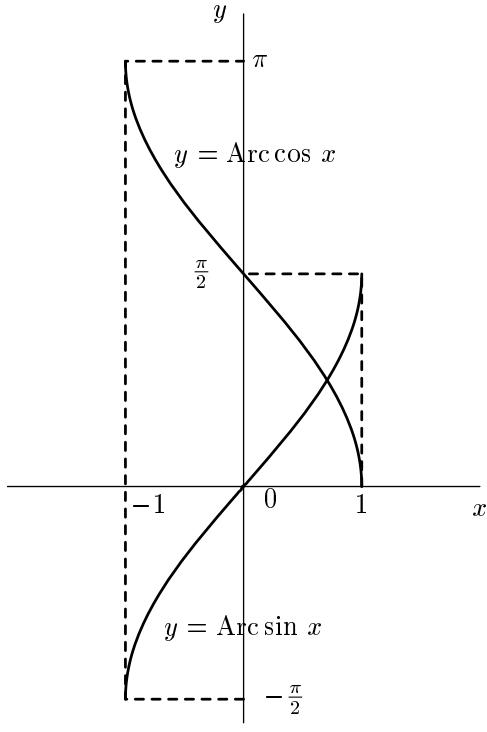
\includegraphics[keepaspectratio]{images/part001_f987f09f.jpg}}\\
图 6

\[
\sin \left(\frac {\pi}{2} - \operatorname{Arc} \cos x\right) = \cos (\operatorname{Arc} \cos x) = x
\]

并且由于 \(-\pi / 2 \leqslant \pi / 2 - \operatorname{Arc} \cos x \leqslant \pi / 2\) ，有

\[
\operatorname{Arc} \cos x = \frac {\pi}{2} - \operatorname{Arc} \sin x\tag{17}
\]

特别由此得出

\[
\mathrm{D} \big (\operatorname{Arc} \cos x \big) = - \frac {1}{\sqrt {1 - x ^ {2}}}.\tag{18}
\]

最后，\(\tan x\) 在区间 \(]-\pi/2, +\pi/2[\) 上的限制是严格递增的；其反函数记作 Arc \(\tan x\) ，它是 R 到 \(]-\pi/2, +\pi/2[\) 上的严格递增映射（图~7）；我们有

\[
\lim _ {x \rightarrow - \infty} \operatorname{Arc} \tan x = - \frac {\pi}{2}, \quad \lim _ {x \rightarrow + \infty} \operatorname{Arc} \tan x = \frac {\pi}{2},
\]

并且，应用反函数求导公式以及 III, p.~95 的公式 (15)，有

\[
\mathrm{D} \big (\operatorname{Arc} \tan x \big) = \frac {1}{1 + x ^ {2}}.\tag{19}
\]

\pandocbounded{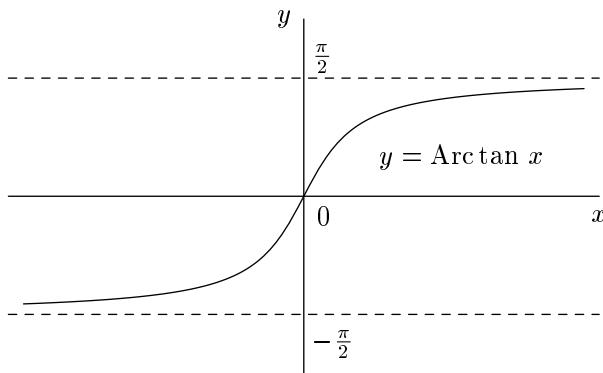
\includegraphics[keepaspectratio]{images/part001_f81b3ea6.jpg}}\\
图 7

\subsection{复指数函数}

我们已在（Gen.~Top., VIII, p.~106）中确定了复数的（加法）拓扑群 C 到（乘法）拓扑群 \(C^{*}\) （由 \(\neq 0\) 的复数组成）上的所有连续同态；它们是映射

\[
x + i y \mapsto e ^ {\alpha x + \beta y} \mathbf {e} (\gamma x + \delta y)\tag{20}
\]

其中 \(\alpha, \beta, \gamma, \delta\) 是满足唯一条件 \(\alpha\delta - \beta\gamma \neq 0\) 的四个实数。我们现在要确定这些同态 \(z \mapsto f(z)\) 中哪些在 C 上可导。首先注意，只需 f 在点 z = 0 可导即可；事实上，对每一点 \(z \in C\) 有 \(\frac{f(z + h) - f(z)}{h} = f(z) \frac{f(h) - 1}{h}\) ；若 \(f'(0)\) 存在，则 \(f'(z)\) 也存在，且 \(f'(z) = af(z)\) ，其中 \(a = f'(0)\) 。另一方面，若 g 是第二个可导同态，满足 \(g'(z) = bg(z)\) ，则 \(g(az/b) = f(z)\) ，因为立即可以看出商 \(g(az/b)/f(z)\) 的导数处处为零且在 z = 0 处等于 1；因此所有可导同态都具有 \(z \mapsto f(\lambda z)\) 的形式，其中 f 是它们中的某一个（假定它们存在），而 \(\lambda\) 是任意（复）常数。

在此情形下，若 \(f\) 在点 \(z = 0\) 可导，则映射 \(x \mapsto f(x)\) 与 \(y \mapsto f(iy)\) （都是 \(\mathbf{R}\) 到 \(\mathbf{C}\) 中的映射）都必在点 0 可导，前者的导数为 \(f'(0)\) ，后者的导数为 \(if'(0)\) 。而映射 \(x \mapsto e^{\alpha x}\mathbf{e}(\gamma x)\) 与 \(y \mapsto e^{\beta y}\mathbf{e}(\delta y)\) 在点 0 的导数分别等于 \(\alpha + 2\pi i\gamma\) 与 \(\beta + 2\pi i\delta\) ，由此得 \(\beta = -2\pi\gamma\) 与 \(\alpha = 2\pi\delta\) ；这些条件特别地为同态 \(x + iy \mapsto e^x\mathbf{e}(y/2\pi)\) 所满足，我们暂时把它记作 \(f_0\) 。现在证明 \(f_0\) 确实在点 \(z = 0\) 可导。

显然 \(x \mapsto f_0(x)\) 与 \(y \mapsto f_0(iy)\) 有各阶导数；特别地，对这两个函数应用 1 阶泰勒公式可知，对每个 \(\varepsilon > 0\) 存在 \(r > 0\) ，使得若令

\[
f _ {0} (x) = 1 + x + \varphi (x) x, \quad f _ {0} (i y) = 1 + i y + \psi (y) y,
\]

则条件 \(|x| \leqslant r, |y| \leqslant r\) 蕴含 \(|\varphi(x)| \leqslant \varepsilon\) 与 \(|\psi(y)| \leqslant \varepsilon\) ；在此情形下，有 \(f_0(x + iy) = f_0(x)f_0(iy) = 1 + (x + iy) + \theta(x, y)\) ，其中

\[
\theta (x, y) = \bigl (i + \varphi (x) \psi (y) \bigr) x y + (1 + x) y \psi (y) + (1 + i y) x \varphi (x);
\]

当 \(|z| \leqslant r\) 时有 \(|x| \leqslant r\) 与 \(|y| \leqslant r\) ，从而

\[
\left| \theta (x, y) \right| \leqslant \left(1 + \varepsilon^ {2}\right) | z | ^ {2} + 2 \varepsilon | z | (1 + | z |)
\]

这证明商 \(\frac{f_{0}(z)-1-z}{z}\) 随 z 趋于 0 而趋于 0 ，也就是说，函数 \(f_{0}\) 在点 z=0 处有导数，等于 1 。于是上面证明了，对一切 \(z\in C\) ，

\[
\mathrm{D} \big (f _ {0} (z) \big) = f _ {0} (z).\tag{21}
\]

这一性质建立了 \(f_{0}\) 与函数 \(e^{x}\) 之间的联系，后者正是 \(f_{0}\) 在实轴上的限制；为此我们给出下面的定义：

定义 2. 同态 \(x + iy \mapsto e^x\mathbf{e}(y/2\pi)\) （\(\mathbf{C}\) 到 \(\mathbf{C}^*\) 上的）称为复指数（函数）；它在任意复数 \(z\) 处的值记作 \(e^z\) 或 \(\exp z\) 。

\subsection{\texorpdfstring{函数 \(e^{z}\) 的性质}{函数 e 的 z 次幂的性质}}

\(z \mapsto e^z\) 是 \(\mathbf{C}\) 到 \(\mathbf{C}^*\) 上的同态，这一事实可用下列恒等式表达

\[
e ^ {z + z ^ {\prime}} = e ^ {z} e ^ {z ^ {\prime}}, \qquad e ^ {0} = 1, \qquad e ^ {- z} = 1 / e ^ {z}.\tag{22}
\]

按定义，对每个 \(z = x + iy\) ，有

\[
e ^ {x + i y} = e ^ {x} (\cos y + i \sin y)\tag{23}
\]

并且由于 \(e^x > 0\) ，可见 \(e^z\) 的绝对值为 \(e^x\) ，辐角为 \(y\) （模 \(2\pi\) ）。

特别地，定义 2（III, p.~98）给出

\[
\mathbf {e} (x) = e ^ {2 \pi i x}\tag{24}
\]

它使我们可以把定义 \(\cos x\) 与 \(\sin x\) 的公式写成如下形式

\[
\cos x = \frac {1}{2} \left(e ^ {i x} + e ^ {- i x}\right), \quad \sin x = \frac {1}{2 i} \left(e ^ {i x} - e ^ {- i x}\right)\tag{25}
\]

（欧拉公式）。

由于 \(2\pi\) 是 \(\mathbf{e}(y/2\pi)\) 的最小周期，\(2\pi i\) 是 \(e^{z}\) 的最小周期；换句话说，\(e^{z}\) 的周期群是数 \(2n\pi i\) 所成的集，其中 n 跑遍 Z。

最后，III, p.~98 的公式 (21) 可写成

\[
\mathrm{D} \left(e ^ {z}\right) = e ^ {z}\tag{26}
\]

从而，对每个复数 \(a\)

\[
\mathrm{D} \big (e ^ {a z} \big) = a e ^ {a z}.\tag{27}
\]

注。若在公式 (27) 中把函数 \(e^{az}\) （a 为复数）限制在实轴上，则对实数 x 再次得到

\[
\mathrm{D} (e ^ {a x}) = a e ^ {a x}.\tag{28}
\]

这个公式使我们可以对 \(e^{\alpha x} \cos \beta x\) ，\(e^{\alpha x} \sin \beta x\) （\(\alpha\) 与 \(\beta\) 为实数）中的每一个函数求出原函数；事实上，我们有 \(e^{(\alpha + i\beta)x} = e^{\alpha x} \cos \beta x + ie^{\alpha x} \sin \beta x\) ，于是由 (28)

\[
\begin{array}{l} \mathrm{D} \left(\mathcal {R} \left(\frac {1}{\alpha + i \beta} e ^ {(\alpha + i \beta) x}\right)\right) = e ^ {\alpha x} \cos \beta x \\ \mathrm{D} \left(\mathcal {I} \left(\frac {1}{\alpha + i \beta} e ^ {(\alpha + i \beta) x}\right)\right) = e ^ {\alpha x} \sin \beta x. \end{array}
\]

同样，可以把求 \(x^n e^{\alpha x} \cos \beta x\) 或 \(x^n e^{\alpha x} \sin \beta x\) （ \(n\) 为整数 \(> 0\) ）的原函数归结为求 \(x^n e^{(\alpha + i\beta)x}\) 的原函数；而 \(n + 1\) 阶分部积分公式（II, p.~60，公式 (11)）表明，后一函数的一个原函数是

\[
e ^ {(\alpha + i \beta) x} \left[ \frac {x ^ {n}}{\alpha + i \beta} - \frac {n x ^ {n - 1}}{(\alpha + i \beta) ^ {2}} + \frac {n (n - 1) x ^ {n - 2}}{(\alpha + i \beta) ^ {3}} + \dots + (- 1) ^ {n} \frac {n !}{(\alpha + i \beta) ^ {n + 1}} \right].
\]

另一方面，利用欧拉公式可以把 \(\cos x\) 或 \(\sin x\) 的每个正整数次幂表示为指数函数 \(e^{ipx}\) （ \(p\) 为正或负整数）的线性组合。于是由公式 (28)，可以把形如 \(x^n e^{\alpha x}(\cos \beta x)^r (\sin \gamma x)^s\) 的函数的原函数表示成形如 \(x^p e^{\alpha x}\cos \lambda x\) 与 \(x^p e^{\alpha x}\sin \mu x\) 的函数的线性组合（\((n, p, r, s\) 为整数，\(\alpha, \beta, \gamma, \lambda, \mu\) 为实数）。

例。有

\[
\sin^ {2 n} x = \frac {(- 1) ^ {n}}{2 ^ {2 n}} \left(e ^ {i x} - e ^ {- i x}\right) ^ {2 n} = \frac {(- 1) ^ {n}}{2 ^ {2 n}} \left(e ^ {2 n i x} - \binom {2 n} {1} e ^ {(2 n - 2) i x} + \dots + e ^ {- 2 n i x}\right)
\]

由此得

\[
\begin{array}{l} \int_ {0} ^ {x} \sin^ {2 n} t d t = \frac {(- 1) ^ {n}}{2 ^ {2 n}} \left(\frac {1}{n} \sin 2 n x - \binom {2 n} {1} \frac {1}{n - 1} \sin (2 n - 2) x + \dots \right. \\ \qquad \qquad \qquad \qquad \qquad \qquad \qquad \qquad \qquad \qquad + (- 1) ^ {n - 1} \binom {2 n} {n - 1} \sin 2 x + (- 1) ^ {n} \binom {2 n} {n} x \Bigg) \end{array}
\]

特别地，

\[
\int_ {0} ^ {\pi / 2} \sin^ {2 n} t   d t = \binom {2 n} {n} \frac {1}{2 ^ {2 n}}   \frac {\pi}{2} = \frac {1 . 3 . 5 \ldots (2 n - 1)}{2 . 4 . 6 \ldots 2 n}   \frac {\pi}{2}.\tag{29}
\]

\subsection{复对数}

设 B 是由点 \(z = x + iy\) （满足 \(-\pi \leqslant y < \pi\) ）所成的“带形”；函数 \(e^{z}\) 在 B 上取它的每个值一次且仅一次；换句话说，\(z \mapsto e^{z}\) 是 B 到 \(C^{*}\) 上的连续双射；在此映射下，（半开）线段 \(x = x_{0}\) ，\(-\pi \leqslant y < \pi\) 的像是圆 \(|z| = e^{x_{0}}\) ；直线 \(y = y_{0}\) 的像是由 \(\operatorname{Am}(z) = y_{0} \pmod{2\pi}\) 定义的（开）半直线。在映射 \(z \mapsto e^{z}\) 下，B 的内部 B （即 \(z \in C\) 中满足 \(|\mathcal{I}(z)| < \pi\) 者所成的集）的像是（闭的）负实半轴在 C 中的余集 F；若约定用 \(\operatorname{Am}(z)\) 表示属于 \([-\pi, \pi]\) 的 z 的辐角量度，则集 F 可由关系 \(-\pi < \operatorname{Am}(z) < \pi\) 定义。由于 \(z \mapsto e^{z}\) 是 C 到 \(C^{*}\) 上的严格同态，任一含于 B 的开集（从而含于 C）在此映射下的像是 \(C^{*}\) 中（从而是 F 中）的开集；换句话说，\(z \mapsto e^{z}\) 在 B 上的限制是 B 到 F 上的同胚。我们把后者的逆同胚，即 F 到 B 上的同胚记作 \(z \mapsto \log z\) ；对复数 \(z \in F\) ，\(\log z\) 称为 z 的对数的主值。若 \(z = x + iy\) 且 \(\log z = u + iv\) ，则 \(x + iy = e^{u + iv}\) ，由此 \(e^{u} = |z|\) ，并且由于 \(-\pi < v < \pi\) ，有 \(v = \operatorname{Am}(z)\) 。此外，有 \(\tan(v + \pi/2) = -x/y\) （若 \(y \neq 0\) ）；于是可以写出

\[
\left\{ \begin{array}{l l} u = \log | z | = \frac {1}{2} \log (x ^ {2} + y ^ {2}) \\ v = \frac {\pi}{2} - \operatorname{Arc} \tan \frac {x}{y} & \text { if } y > 0 \\ v = 0 & \text { if } y = 0 \\ v = - \frac {\pi}{2} - \operatorname{Arc} \tan \frac {x}{y} & \text { if } y <   0. \end{array} \right.\tag{30}
\]

显然 \(\log z\) 是函数 \(\log x\) （定义在正开实半轴 \(R_{+}^{*}\) 上）到 F 上的延拓。若 z，\(z'\) 是 F 中使 \(zz'\) 非负实数的两点，则有 \(\log(zz') = \log z + \log z' + 2\varepsilon\pi i\) ，其中 \(\varepsilon = +1\) 、-1 或 0，视 \(\mathrm{Am}(z)\) 与 \(\mathrm{Am}(z')\) 的值而定。

我们注意，在负实半轴的各点处函数 \(\log z\) 没有极限；确切地说，若 x 趋于 \(x_{0} < 0\) 且 y 保持 \textgreater{} 0（相应地，\textless{} 0）地趋于 0，则 \(\log z\) 趋于 \(\log |x_{0}| + \pi i\) （相应地，\(\log |x_{0}| - \pi i\) ）；当 z 趋于 0 时，\(|\log z|\) 无限增大。

以后我们将看到，解析函数理论如何使我们能把函数 \(\log z\) 延拓，并在完全一般的意义下定义复对数。

由于 \(\log z\) 是 \(e^{z}\) 的逆同胚，反函数求导公式（I, p.~9, prop. 6）表明 \(\log z\) 在每一点 \(z \in F\) 处可导，并且

\[
\mathrm{D} (\log z) = \frac {1}{e ^ {\log z}} = \frac {1}{z}\tag{31}
\]

这个公式推广了 III, p.~93 的公式 (10)。

\subsection{有理函数的原函数}

公式 (31) 使我们能够求出实变量 x 的任意有理函数 \(r(x)\) （系数为实的或复的）的原函数。我们知道（A.VII.7），这样的函数可以（以唯一的方式）写成有限多项之和，这些项是：

\begin{enumerate}
\def\labelenumi{\alph{enumi})}
\item
  或者形如 \(ax^{p}\) （p 为整数 \(\geqslant 0\) ，a 为复数）；
\item
  或者形如 \(a/(x - b)^{m}\) （m 为整数 \(\geqslant 0\) ，a 与 b 为复数）。
\end{enumerate}

现在，容易求出其中每一项的原函数：

\begin{enumerate}
\def\labelenumi{\alph{enumi})}
\tightlist
\item
  \(ax^p\) 的原函数是 \(a\frac{x^{p + 1}}{p + 1}\) ；
\end{enumerate}

\(b)\) 若 \(m > 1\) ，\(a / (x - b)^{m}\) 的原函数是 \(\frac{a}{(1 - m)(x - b)^{m - 1}}\) ；

\begin{enumerate}
\def\labelenumi{\alph{enumi})}
\setcounter{enumi}{2}
\tightlist
\item
  最后，由公式 (10)（III, p.~93）与 (31)（III, p.~101），\(\frac{a}{x - b}\) 的原函数是 \(a\log |x - b|\) （若 \(b\) 为实数），是 \(a\log (x - b)\) （若 \(b\) 为复数）。在后一情形，若 \(b = p + iq\) ，则还有（III, p.~100，公式 (30)）
\end{enumerate}

\[
\log (x - b) = \log \sqrt {(x - p) ^ {2} + q ^ {q}} + i \operatorname{Arc} \tan \frac {x - p}{q} \pm i \frac {\pi}{2}.
\]

我们把更实用的、明显地求出显式给出的有理函数的原函数的方法的考察，推迟到本丛书专讲数值计算的部分。

下列求原函数的问题都可以归结为求有理函数的原函数：

\(1^{\circ}\) 求形如 \(r(e^{ax})\) 的函数的原函数，其中 \(r\) 是有理函数而 \(a\) 是实数；事实上，通过变量替换 \(u = e^{ax}\) ，可归结为求 \(r(u) / u\) 的原函数；

\(2^{\circ}\) 求形如 \(f(\sin ax, \cos ax)\) 的函数的原函数，其中 \(f\) 是两个变量的有理函数而 \(a\) 是实数；变量替换 \(u = \tan(ax/2)\) 把它归结为求下列函数的原函数

\[
{\frac {2}{1 + u ^ {2}}} f \left({\frac {2 u}{1 + u ^ {2}}}, {\frac {1 - u ^ {2}}{1 + u ^ {2}}}\right).
\]

\subsection{复圆函数；双曲函数}

欧拉公式 (25)（III, p.~99）与 \(e^z\) （对每个复数 \(z\) 而言）的定义，使我们可以向 \(\mathbf{C}\) 延拓函数 \(\cos x\) 与 \(\sin x\) ——它们定义在 \(\mathbf{R}\) 上——，只需对一切 \(z \in \mathbf{C}\) 令

\[
\cos z = \frac {1}{2} \left(e ^ {i z} + e ^ {- i z}\right), \quad \sin z = \frac {1}{2 i} \left(e ^ {i z} - e ^ {- i z}\right)\tag{32}
\]

（cf.~III, p.~119, exerc. 19）。

这些函数是以 \(2\pi\) 为最小周期的周期函数；即有 \(\cos(z + \pi/2) = -\sin z\) ，\(\sin(z + \pi/2) = \cos z\) ；还可以验证恒等式

\[
\begin{array}{c} \cos^ {2} z + \sin^ {2} z = 1 \\ \cos (z + z ^ {\prime}) = \cos z \cos z ^ {\prime} - \sin z \sin z ^ {\prime} \\ \sin (z + z ^ {\prime}) = \sin z \cos z ^ {\prime} + \cos z \sin z ^ {\prime}. \end{array}
\]

更一般地，实变量圆函数之间的每个代数恒等式当这些变量取任意复值时仍然成立（III, p.~119, exerc. 18）。

令 \(\tan z = \sin z/\cos z\) （若 \(z \neq (2k + 1)\pi/2\) ），令 \(\cot z = \cos z/\sin z\) （若 \(z \neq k\pi\) ）；它们是以 \(\pi\) 为最小周期的周期函数。

公式 (27)（III, p.~99）表明 \(\cos z\) 与 \(\sin z\) 在 \(\mathbf{C}\) 上可导，并且

\[
\mathrm{D} (\cos z) = - \sin z, \quad \mathrm{D} (\sin z) = \cos z.
\]

对 \(z = ix\) （x 为实数），公式 (32) 给出

\[
\cos i x = \frac {1}{2} \left(e ^ {x} + e ^ {- x}\right), \quad \sin i x = \frac {i}{2} \left(e ^ {x} - e ^ {- x}\right).
\]

对这样引入的实函数，采用专门的记号是方便的；我们令

\[
\left\{ \begin{array}{l l} \cosh x = \frac {1}{2} \left(e ^ {x} + e ^ {- x}\right) & \text {(hyperbolic cosine of x)} \\ \sinh x = \frac {i}{2} \left(e ^ {x} - e ^ {- x}\right) & \text {(hyperbolic sine of x)} \\ \tanh x = \frac {\sinh x}{\cosh x} = \frac {e ^ {x} - e ^ {- x}}{e ^ {x} + e ^ {- x}} & \text {(hyperbolic tangent of x)} \end{array} \right.\tag{33}
\]

于是，对每个实数 \(x\)

\[
\cos i x = \cosh x, \quad \sin i x = i \sinh x.\tag{34}
\]

由若干复数 \(z_{k}\) （ \(1 \leqslant k \leqslant n\) ）的圆函数之间的每个恒等式，把 \(z_{k}\) 换成 \(ix_{k}\) （ \(x_{k}\) 为实数，\(1 \leqslant k \leqslant n\) ）并利用公式 (34)，就可以得到双曲函数的一个恒等式；例如有

\[
\begin{array}{c} \cosh^ {2} x - \sinh^ {2} x = 1 \\ \cosh (x + x ^ {\prime}) = \cosh x \cosh x ^ {\prime} + \sinh x \sinh x ^ {\prime} \\ \sinh (x + x ^ {\prime}) = \sinh x \cosh x ^ {\prime} - \cosh x \sinh x ^ {\prime}. \end{array}
\]

双曲函数使我们可以表出 \(\cos z\) 与 \(\sin z\) 当 \(z = x + iy\) 时的实部与虚部，因为

\[
\begin{array}{l} \cos (x + i y) = \cos x \cos i y - \sin x \sin i y = \cos x \cosh y - i \sin x \sinh y \\ \sin (x + i y) = \sin x \cos i y + \cos x \sin i y = \sin x \cosh y + i \cos x \sinh y. \end{array}
\]

最后，有

\[
\mathrm{D} (\cosh x) = \sinh x, \mathrm{D} (\sinh x) = \cosh x, \mathrm{D} (\tanh x) = 1 - \tanh ^ {2} x = \frac {1}{\cosh^ {2} x}.
\]

由于对一切 x 有 \(\cosh x > 0\) ，由此推出 \(\sinh x\) 在 R 上严格递增；又 \(\sinh 0 = 0\) ，故 \(\sinh x\) 与 x 同号。于是 \(\cosh x\) 在 \(x \leqslant 0\) 时严格递减，在 \(x \geqslant 0\) 时严格递增；最后，\(\tanh x\) 在 R 上严格递增。此外

\[
\begin{array}{l} \lim _ {x \to - \infty} \sinh x = - \infty , \quad \lim _ {x \to + \infty} \sinh x = + \infty \\ \lim _ {x \to - \infty} \cosh x = \lim _ {x \to + \infty} \cosh x = + \infty \\ \lim _ {x \to - \infty} \tanh x = - 1, \quad \lim _ {x \to + \infty} \tanh x = + 1 \quad (\text {   fig.   8   and   9   }). \end{array}
\]

有时以 \(\operatorname{Arg}\sinh x\) 表示 \(\sinh x\) 的反函数，它是 \(\mathbf{R}\) 到 \(\mathbf{R}\) 上的严格递增映射；这个函数也可以用对数表示，因为由关系式 \(x = \sinh y = \frac{1}{2}(e^y - e^{-y})\) 推出 \(e^{2y} - 2xe^y - 1 = 0\) ，而由于 \(e^y > 0\) ，有 \(e^y = x + \sqrt{x^2 + 1}\) ，也就是说

\[
\operatorname{Arg} \sinh x = \log (x + \sqrt {x ^ {2} + 1}).
\]

类似地，我们把 \(\operatorname{Arg}\cosh x\) 记为 \(\cosh x\) 在 \([0, +\infty[\) 上的限制的反函数；这个映射是 \([1, +\infty[\) 到 \([0, +\infty[\) 上的严格递增映射；与上面一样可以证明

\[
\operatorname{Arg} \cosh x = \log (x + \sqrt {x ^ {2} - 1}).
\]

\pandocbounded{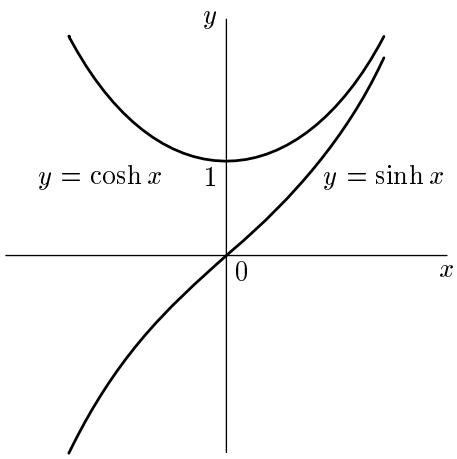
\includegraphics[keepaspectratio]{images/part001_d9e35212.jpg}}\\
图 8

\pandocbounded{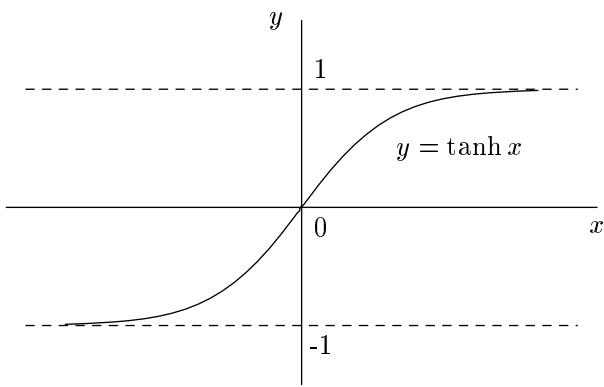
\includegraphics[keepaspectratio]{images/part001_f5896466.jpg}}\\
图 9

最后，我们以 \(\operatorname{Arg}\tanh x\) 表示 \(\tanh x\) 的反函数，它是 \(] - 1, +1[\) 到 \(\mathbf{R}\) 上的严格递增映射；此外有

\[
\operatorname{Arg} \tanh x = \frac {1}{2} \log \frac {1 + x}{1 - x}.
\]

注。对复数 \(z\) ，有时写

\[
\begin{array}{l} \cosh z = \frac {1}{2} (e ^ {z} + e ^ {- z}) = \cos i z \\ \sinh z = \frac {1}{2} (e ^ {z} - e ^ {- z}) = - i \sin i z. \end{array}
\]

这些函数就这样把定义在 R 上的双曲函数延拓到了 C。

\section{指数函数、圆函数及其相关函数的展开}

\subsection{实指数函数的展开}

由于 \(\mathrm{D}^n (e^x) = e^x\) ，按 \(n\) 阶泰勒展开，\(e^x\) 为

\[
e ^ {x} = 1 + \frac {x}{1 !} + \frac {x ^ {2}}{2 !} + \dots + \frac {x ^ {n}}{n !} + \int_ {0} ^ {x} \frac {(x - t) ^ {n}}{n !} e ^ {t} d t.\tag{1}
\]

这个公式的余项 \(>0\) （当 \(x > 0\) ），且有 \((-1)^{n + 1}\) 的符号（当 \(x < 0\) ）；此外，中值不等式表明

\[
\frac {x ^ {n + 1}}{(n + 1) !} <   \int_ {0} ^ {x} \frac {(x - t) ^ {n}}{n !} e ^ {t} d t <   \frac {x ^ {n + 1} e ^ {x}}{(n + 1) !} \quad \text { for } x > 0\tag{2}
\]

\[
\frac {\left| x ^ {n + 1} \right| e ^ {x}}{(n + 1) !} <   \left| \int_ {0} ^ {x} \frac {(x - t) ^ {n}}{n !} e ^ {t} d t \right| <   \frac {\left| x ^ {n + 1} \right|}{(n + 1) !} \quad \text { for } x <   0\tag{3}
\]

现在我们知道，序列 \((x^{n}/n!)\) 当 n 无限增大时以 0 为极限（对一切 \(x \geqslant 0\) ；Gen.~Top., IV, p.~365）；于是，在 (1) 中固定 x 而让 n 无限增大，由 (2) 与 (3) 就得出

\[
e ^ {x} = \sum_ {n = 0} ^ {\infty} \frac {x ^ {n}}{n !}\tag{4}
\]

并且右端的级数在 \(\mathbf{R}\) 的每个紧区间上绝对且一致收敛。特别地，有公式

\[
e = 1 + \frac {1}{1 !} + \frac {1}{2 !} + \dots + \frac {1}{n !} + \dots\tag{5}
\]

这个公式使我们可以计算出与数 \(e\) 任意接近的有理近似值；我们得到

\[
e = 2. 7 1 8   2 8 1   8 2 8 \dots
\]

精确到 \(1/10^{9}\) 。此外，公式 (5) 证明 e 是无理数 \(^{2}\) （Gen.~Top., IV, p.~375）。

注。由于公式 (1) 的余项 \textgreater0 （当 x \textgreater{} 0 时），故对 x \textgreater{} 0 有

\[
e ^ {x} > 1 + \frac {x}{1 !} + \frac {x ^ {2}}{2 !} + \dots + \frac {x ^ {n + 1}}{(n + 1) !}
\]

因而更有

\[
e ^ {x} > \frac {x ^ {n + 1}}{(n + 1) !}
\]

对每个整数 \(n\) 成立：由此推出，\(e^x / x^n\) 以 \(+\infty\) 为极限（当 \(x\) 无限增大时；对每个整数 \(n\) ）：我们将在第 V 章中用另一种方法再次得到这一结果（V, p.~231）。

\subsection{\texorpdfstring{复指数函数、\(\cos x\) 与 \(\sin x\) 的展开。}{复指数函数、cos x 与 sin x 的展开。}}

设 z 是任意复数，考虑实变量 t 的函数 \(\varphi(t) = e^{zt}\) ；我们有 \(\mathrm{D}^{n}\varphi(t) = z^{n}e^{zt}\) 与 \(e^{z} = \varphi(1)\) ；于是，用 \(\varphi(1)\) 在点 t = 0 处的 n 阶泰勒公式来表示它（II, p.~62），便得

\[
e ^ {z} = 1 + \frac {z}{1 !} + \frac {z ^ {2}}{2 !} + \dots + \frac {z ^ {n}}{n !} + z ^ {n + 1} \int_ {0} ^ {1} \frac {(1 - t) ^ {n}}{n !} e ^ {z t} d t\tag{6}
\]

当 \(z\) 为实数时这个公式与 (1) 等价。余项

\[
r _ {n} (z) = z ^ {n + 1} \int_ {0} ^ {1} \frac {(1 - t) ^ {n}}{n !} e ^ {z t} d t
\]

的绝对值可用中值不等式从上方控制；若 \(z = x + iy\) ，我们有 \(|e^{zt}| = e^{xt}\) ，于是 \(|e^{zt}| \leqslant 1\) （当 \(x \leqslant 0\) ），\(|e^{zt}| \leqslant e^x\) （当 \(x > 0\) ）；因此

\[
\left| r _ {n} (z) \right| \leqslant \frac {\left| z \right| ^ {n + 1}}{(n + 1) !} \text {   if   } x \leqslant 0\tag{7}
\]

\[
| r _ {n} (z) | \leqslant \frac {| z | ^ {n + 1} e ^ {x}}{(n + 1) !} \text {   if   } x > 0.\tag{8}
\]

与上面一样，我们得出

\[
e ^ {z} = \sum_ {n = 0} ^ {\infty} \frac {z ^ {n}}{n !}\tag{9}
\]

该级数在 \(\mathbf{C}\) 的每个紧子集上绝对且一致收敛。由 (6) 特别得出

\[
e ^ {i x} = 1 + \frac {i x}{1 !} + \frac {i ^ {2} x ^ {2}}{2 !} + \dots + \frac {i ^ {n} x ^ {n}}{n !} + i ^ {n + 1} \int_ {0} ^ {x} \frac {(x - t) ^ {n}}{n !} e ^ {i t} d t\tag{10}
\]

由此可得 \(\cos x\) 与 \(\sin x\) 的泰勒展开；取 (10) 的 \(2n + 1\) 阶实部便得

\[
\cos x = 1 - \frac {x ^ {2}}{2 !} + \dots + (- 1) ^ {n} \frac {x ^ {2 n}}{(2 n) !} + (- 1) ^ {n + 1} \int_ {0} ^ {x} \frac {(x - t) ^ {2 n + 1}}{(2 n + 1) !} \cos t d t\tag{11}
\]

其余项满足界

\[
\left| \int_ {0} ^ {x} \frac {(x - t) ^ {2 n + 1}}{(2 n + 1) !} \cos t d t \right| \leqslant \frac {| x | ^ {2 n + 2}}{(2 n + 2) !}.\tag{12}
\]

类似地，取 (10) 的 \(2n\) 阶虚部，我们得到

\[
\begin{array}{l} \sin x = x - \frac {x ^ {3}}{3 !} + \frac {x ^ {5}}{5 !} + \dots + (- 1) ^ {n - 1} \frac {x ^ {2 n - 1}}{(2 n - 1) !} \\ \qquad + (- 1) ^ {n} \int_ {0} ^ {x} \frac {(x - t) ^ {2 n}}{(2 n) !} \cos t d t \end{array}\tag{13}
\]

其余项满足界

\[
\left| \int_ {0} ^ {x} \frac {(x - t) ^ {2 n}}{(2 n) !} \cos t d t \right| \leqslant \frac {| x | ^ {2 n + 1}}{(2 n + 1) !}.\tag{14}
\]

此外，比较 (11) 中 \(2n + 1\) 阶与 \(2n + 3\) 阶的余项，有

\[
\int_ {0} ^ {x} \frac {(x - t) ^ {2 n + 3}}{(2 n + 3) !} \cos t d t = \frac {x ^ {2 n + 2}}{(2 n + 2) !} - \int_ {0} ^ {x} \frac {(x - t) ^ {2 n + 1}}{(2 n + 1) !} \cos t d t
\]

并把 (12) 考虑在内，便知不论 x 为何值，(11) 的余项都有与 \((-1)^{n+1}\) 相同的符号；同样可以证明 (13) 的余项与 \((-1)^{n}x\) 同号。特别地，在 (11) 中取 n = 0 与 n = 1，在 (13) 中取 n = 1 与 n = 2，就得到不等式

\[
1 - \frac {x ^ {2}}{2} \leqslant \cos x \leqslant 1 \quad \text { for   all } x\tag{15}
\]

\[
x - \frac {x ^ {3}}{6} \leqslant \sin x \leqslant x \quad \text { for   all } x \geqslant 0.\tag{16}
\]

最后，在 (9) 中令 z = ix 便得

\[
\cos x = \sum_ {n = 0} ^ {\infty} (- 1) ^ {n} \frac {x ^ {2 n}}{(2 n) !}\tag{17}
\]

\[
\sin x = \sum_ {n = 0} ^ {\infty} (- 1) ^ {n} \frac {x ^ {2 n + 1}}{(2 n + 1) !}\tag{18}
\]

这些级数在每个紧区间上绝对且一致收敛。

此外，显然公式 (17) 与 (18) 对每个复数 x 仍然成立，右端的级数在 C 的每个紧子集上绝对且一致收敛。特别地，对每个 x（实的或复的）

\[
\begin{array}{l} \cosh x = \sum_ {n = 0} ^ {\infty} \frac {x ^ {2 n}}{(2 n) !} \\ \sinh x = \sum_ {n = 0} ^ {\infty} \frac {x ^ {2 n + 1}}{(2 n + 1) !}. \end{array}
\]

\subsection{二项展开}

设 \(m\) 是任意实数。对 \(x > 0\) 我们有

\[
\mathrm{D} ^ {n} (x ^ {m}) = m (m - 1) \dots (m - n + 1) x ^ {m - n};
\]

把 \(n\) 阶泰勒公式（关于点 \(x = 0\) ）应用于函数 \((1 + x)^m\) ，便知对每个 \(x > -1\)

\[
(1 + x) ^ {m} = 1 + \binom {m} {1} x + \binom {m} {2} x ^ {2} + \dots + \binom {m} {n} x ^ {n} + r _ {n} (x)\tag{19}
\]

其中

\[
r _ {n} (x) = \frac {m (m - 1) \dots (m - n)}{n !} \int_ {0} ^ {x} \left(\frac {x - t}{1 + t}\right) ^ {n} (1 + t) ^ {m - 1} d t
\]

其中令 \(\binom{m}{n} = \frac{m(m-1)\ldots(m-n+1)}{n!}\) 。当 m 是整数 \textgreater{} 0 且 \(n \geqslant m\) 时，公式 (19) 就化为二项式公式（Alg., I, p.~99）；通过推广，我们仍称它为二项式公式，并称系数 \(\binom{m}{n}\) 为二项式系数，这里 m 是任意实数而 n 是任意整数 \textgreater{} 0 。

(19) 的余项与 \(\binom{m}{n+1}\) 同号（当 \(x > 0\) 时），且与 \((-1)^{n+1}\binom{m}{n+1}\) 同号（当 \(-1 < x < 0\) 时）。由于 \(\left|\frac{x-t}{1+t}\right| \leqslant |x|\) 对 \(t > -1\) （在以 0 与 \(x\) 为端点的区间中）成立，故对任意的 \(m\) 、\(n\) 与 \(x > -1\) ，余项满足下面的界：

\[
\begin{array}{r l} \left| \frac {m (m - 1) \dots (m - n)}{n !} \int_ {0} ^ {x} \left(\frac {x - t}{1 + t}\right) ^ {n} (1 + t) ^ {m - 1} d t \right| & \\ & \leqslant \left| \binom {m - 1} {n} x ^ {n} ((1 + x) ^ {m} - 1) \right|. \end{array}\tag{20}
\]

若设 \(x \geqslant 0\) 且 \(n \geqslant m - 1\) ，则在积分区间上 \((1 + t)^{n - m + 1} \geqslant 1\) ，于是

\[
0 \leqslant \int_ {0} ^ {x} \frac {(x - t) ^ {n}}{(1 + t) ^ {n - m + 1}} d t \leqslant \int_ {0} ^ {x} (x - t) ^ {n} d t = \frac {x ^ {n + 1}}{n + 1}
\]

由此得到估计式

\[
\left| r _ {n} (x) \right| \leqslant \left| \binom {m} {n + 1} \right| x ^ {n + 1} \quad (x \geqslant 0, n \geqslant m - 1)\tag{21}
\]

它是对余项的估计。另一方面，设 \(-1 \leqslant m < 0\) ；若在积分 (19) 中作变量替换 \(u = \frac{x - t}{x(1 + t)}\) ，则得

\[
r _ {n} (x) = \frac {m (m - 1) \dots (m - n)}{n !} (1 + x) ^ {m} x ^ {n + 1} \int_ {0} ^ {1} \frac {u ^ {n} d u}{(1 + u x) ^ {m + 1}}.\tag{22}
\]

为对 x \textgreater{} -1 的情形估计该积分，我们注意到：由于 \(m + 1 < 1\) ，积分 \(\int_{0}^{1}\frac{u^{n}du}{(1-u)^{m+1}}\) 收敛，且因 \(1+ux > 1-u\) ，它控制 (22) 的右端。而对 -1 \textless{} x \textless{} 0 ，关于 m 的假设蕴含 (19) 右端出现的所有项 \(\binom{m}{1}x,\binom{m}{2}x^{2},\ldots,\binom{m}{n}x^{n}\) 均 \(\geqslant 0\) ，故 \(r_{n}(x) \leqslant (1+x)^{m}\) ；用 \((1+x)^{m}\) 除之，即得

\[
\frac {m (m - 1) \dots (m - n)}{n !} x ^ {n + 1} \int_ {0} ^ {1} \frac {u ^ {n} d u}{(1 + u x) ^ {m + 1}} \leqslant 1.
\]

此外，当 \(-1 < x < 0\) 时积分号前的因子 \(\geqslant 0\) ，故令 \(x\) 趋于 \(-1\) ，便得

\[
\left| \frac {m (m - 1) \dots (m - n)}{n !} \int_ {0} ^ {1} \frac {u ^ {n} d u}{(1 - u) ^ {m + 1}} \right| \leqslant 1
\]

因而当 \(-1 \leqslant m < 0\) 且 \(x > -1\) 时有

\[
\left| r _ {n} (x) \right| \leqslant (1 + x) ^ {m} | x | ^ {n + 1}.\tag{23}
\]

首先，从这些不等式可以推出：当 \(|x| < 1\) 时有

\[
(1 + x) ^ {m} = \sum_ {n = 0} ^ {\infty} \binom {m} {n} x ^ {n}\tag{24}
\]

其右端（称为二项级数）在 {]} - 1, +1{[} 的每个紧子集上绝对且一致收敛。事实上，可以写出

\[
\binom {m} {n} = (- 1) ^ {n} \left(1 - \frac {m + 1}{1}\right) \left(1 - \frac {m + 1}{2}\right) \dots \left(1 - \frac {m + 1}{n}\right)\tag{25}
\]

由此得

\[
\left| \binom {m} {n} \right| \leqslant \left(1 + \frac {| m + 1 |}{1}\right) \left(1 + \frac {| m + 1 |}{2}\right) \dots \left(1 + \frac {| m + 1 |}{n}\right).
\]

若 \(|x| \leqslant r < 1\) ，则存在 \(n_0\) 使得 \(1 + \frac{|m|}{n_0} < \frac{1}{r'}\) ，其中 \(r < r' < 1\) ；由此，令

\[
k = \left(1 + \frac {| m |}{1}\right) \left(1 + \frac {| m |}{2}\right) \dots \left(1 + \frac {| m |}{n _ {0}}\right)
\]

便有

\[
\left| \binom {m - 1} {n} x ^ {n} \right| \leqslant k | x | ^ {n _ {0}} \left(\frac {r}{r ^ {\prime}}\right) ^ {n - n _ {0}},
\]

这就证明了该命题。另一方面，对 x \textgreater{} 1 ，若 m 不是整数 \(\geqslant 0\) ，则级数 (24) 通项的绝对值随 n 无限增大；事实上，由 (25) 知，对 \(n > n_{1} \geqslant |m + 1|\) 有

\[
\begin{array}{r l} \left| \binom {m} {n} \right| & \geqslant \left| \left(1 - \frac {m + 1}{1}\right) \left(1 - \frac {m + 1}{2}\right) \dots \left(1 - \frac {m + 1}{n _ {1}}\right) \right| \\ & \quad \left(1 - \frac {| m + 1 |}{n _ {1} + 1}\right) \dots \left(1 - \frac {| m + 1 |}{n}\right). \end{array}
\]

取 \(n_0 \geqslant n_1\) 使得当 \(n \geqslant n_0\) 时 \(1 - \frac{|m + 1|}{n} > \frac{1}{x'}\) ，其中 \(1 < x' < x\) 。若令

\[
k ^ {\prime} = \left| \left(1 - \frac {m + 1}{1}\right) \dots \left(1 - \frac {m + 1}{n _ {1}}\right) \right| \left(1 - \frac {| m + 1 |}{n _ {1} + 1}\right) \dots \left(1 - \frac {| m + 1 |}{n _ {0}}\right)
\]

则当 \(n > n_0\) 时

\[
\left| \binom {m} {n} x ^ {n} \right| \geqslant k ^ {\prime} | x | ^ {n _ {0}} \left(\frac {x}{x ^ {\prime}}\right) ^ {n - n _ {0}}
\]

命题由此得证。

我们注意到，当 \(m = -1\) 时，代数恒等式

\[
\frac {1}{1 + x} = 1 - x + x ^ {2} - \dots + (- 1) ^ {n - 1} x ^ {n - 1} + (- 1) ^ {n} \frac {x ^ {n}}{1 + x}\tag{26}
\]

无需积分便给出了普遍公式 (19) 中余项的表达式；这时公式 (23) 化为几何级数（或等比数列）求和的表达式（Gen.~Top., IV, p.~364）。

其次，我们来研究二项级数当 \(x = 1\) 或 \(x = -1\) 时的收敛性（排除平凡情形 \(m = 0\) ）：

\begin{enumerate}
\def\labelenumi{\alph{enumi})}
\item
  \(m \leqslant -1\) 。通项为 \(1 - \frac{m + 1}{n}\) 的乘积趋于 \(+\infty\) （若 \(m < -1\) ），趋于 1 （若 \(m = -1\) ），故由 (25) 知，当 \(x = \pm 1\) 时二项级数的通项不趋于 0。
\item
  -1 \textless{} m \textless{} 0。这时通项为 \(1 - \frac{m + 1}{n}\) 的乘积趋于 0 ，故不等式 (21) 表明 \(r_{n}(1)\) 趋于 0。于是二项级数在 x = 1 处收敛且和为 \(2^{m}\) ；此外，由前文所见及 (21) ，二项级数在每个区间 \([x_{0}, 1]\) （ \(-1 < x_{0} \leqslant 1\) ）上一致收敛。另一方面，当 x = -1 时 (24) 右端所有的项都 \(\geqslant 0\) ；倘若这级数收敛，便可推出二项级数在 \([-1, 1]\) 上正规收敛，从而其和是该区间上的连续函数，而这是荒谬的，因为 \((1 + x)^{m}\) 在 \([-1, 1]\) 上无界（当 m \textless{} 0 时）。由此断定，二项级数在 x = 1 处同样不是绝对收敛的。
\item
  m \textgreater{} 0。\(r_{n}(x)\) 的定义表明，当 x 趋于 -1 时 \(r_{n}(x)\) 趋于极限 \(r_{n}(-1)\) ；在 (20) 中取极限便可断定 \(|r_{n}(-1)| \leqslant \left|\binom{m-1}{n}\right|\) ，又因 m - 1 \textgreater{} -1 ，可见二项级数在 x = -1 处收敛。此外，当 \(n > m + 1\) 时该级数所有的项同号；因而二项级数在区间 \([-1, 1]\) 上正规收敛，且在该区间上的和为 \((1 + x)^{m}\) 。
\end{enumerate}

\subsection{\texorpdfstring{\(\log(1 + x)\)、Arc tan x 与 Arc sin x 的展开}{log(1 + x)、Arc tan x 与 Arc sin x 的展开}}

将 (26) 两端从 0 到 x 积分，即得 \(\log(1 + x)\) 的 n 阶泰勒展开，它对 x \textgreater{} -1 成立

\[
\log (1 + x) = \frac {x}{1} - \frac {x ^ {2}}{2} + \frac {x ^ {3}}{3} + \dots + (- 1) ^ {n - 1} \frac {x ^ {n}}{n} + (- 1) ^ {n} \int_ {0} ^ {x} \frac {t ^ {n} d t}{1 + t}.\tag{27}
\]

余项与 \((-1)^{n}\) 同号（当 x \textgreater{} 0 时），且为 \textless{} 0 （当 -1 \textless{} x \textless{} 0 时）；再者，当 x \textgreater{} 0 时，有 \(1 + t \geqslant 1\) （对 \(0 \leqslant t \leqslant x\) ），而当 -1 \textless{} x \textless{} 0 时，有 \(1 + t \geqslant 1 - |x|\) （对 \(x \leqslant 0\) ）；由此得余项的估计式

\[
\left| \int_ {0} ^ {x} \frac {t ^ {n} d t}{1 + t} \right| \leqslant \frac {| x | ^ {n + 1}}{n + 1}
\]

\[
\text { for } x \geqslant 0\tag{28}
\]

\[
\left| \int_ {0} ^ {x} \frac {t ^ {n} d t}{1 + t} \right| \leqslant \frac {| x | ^ {n + 1}}{(n + 1) (1 - | x |)} \quad \text {   for   } - 1 <   x \leqslant 0.\tag{29}
\]

由最后这两个公式立即可得：当 \(-1 < x \leqslant 1\) 时有

\[
\log (1 + x) = \sum_ {n = 1} ^ {\infty} (- 1) ^ {n - 1} \frac {x ^ {n}}{n}\tag{30}
\]

该级数在含于 \(]-1,+1]\) 的每个紧区间上一致收敛，且当 \(|x|<1\) 时绝对收敛。

另一方面，当 \(|x| > 1\) 时 (30) 右端级数的通项的绝对值随 n 无限增大（III, p.~106）。当 x = -1 时该级数化为调和级数，其和为 \(+\infty\) （Gen.~Top., IV, p.~365）。

类似地，在 (26) 中把 \(x\) 换成 \(x^2\) ，并将两端从 0 到 \(x\) 积分，即得 \(2n - 1\) 阶泰勒展开（对 \(\operatorname{Arctan} x\) ），它对一切实数 \(x\) 成立

\[
\operatorname{Arc} \tan x = \frac {x}{1} - \frac {x ^ {3}}{3} + \frac {x ^ {5}}{5} + \dots + (- 1) ^ {n - 1} \frac {x ^ {2 n - 1}}{2 n - 1} + (- 1) ^ {n} \int_ {0} ^ {x} \frac {t ^ {2 n} d t}{1 + t ^ {2}}.\tag{31}
\]

余项与 \((-1)^n x\) 同号；由于 \(1 + t^2 \geqslant 1\) 对一切 \(t\) 成立，我们有估计式

\[
\left| \int_ {0} ^ {x} \frac {t ^ {2 n} d t}{1 + t ^ {2}} \right| \leqslant \frac {| x | ^ {2 n + 1}}{2 n + 1}\tag{32}
\]

由此推出：当 \(|x| \leqslant 1\) 时

\[
\operatorname{Arc} \tan x = \sum_ {n = 1} ^ {\infty} (- 1) ^ {n - 1} \frac {x ^ {2 n - 1}}{2 n - 1}\tag{33}
\]

该级数在 \([-1,+1]\) 上一致收敛，且当 \(|x|<1\) 时绝对收敛。

特别地，取 \(x = 1\) 便得到公式

\[
{\frac {\pi}{4}} = 1 - {\frac {1}{3}} + {\frac {1}{5}} + \dots + (- 1) ^ {n} {\frac {1}{2 n + 1}} + \dots .\tag{34}
\]

当 \(|x| > 1\) 时 (33) 右端的通项的绝对值随 \(n\) 无限增大。

最后，关于 Arc sin x 的泰勒展开，我们从其导数 \((1 - x^{2})^{-1/2}\) 的展开出发；后一展开是在二项级数展开中以 \(-x^{2}\) 代换 x 而从 \((1 + x)^{-1/2}\) 得到的；对 \(|x| < 1\) 这给出

\[
(1 - x ^ {2}) ^ {- 1 / 2} = 1 + \frac {1}{2} x ^ {2} + \frac {1 . 3}{2 . 4} x ^ {4} + \dots + \frac {1 . 3 . 5 \dots (2 n - 1)}{2 . 4 . 6 \dots 2 n} x ^ {2 n} + r _ {n} (x)
\]

并且由 (23) ，其余项满足界

\[
0 \leqslant r _ {n} (x) \leqslant \frac {x ^ {2 n + 2}}{\sqrt {1 - x ^ {2}}}
\]

此即对余项的界。

取前一展开式的原函数，便得

\[
\operatorname{Arc} \sin x = x + \frac {1}{2} \frac {x ^ {3}}{3} + \frac {1 . 3}{2 . 4} \frac {x ^ {5}}{5} + \dots + \frac {1 . 3 . 5 \dots (2 n - 1)}{2 . 4 . 6 \dots 2 n} \frac {x ^ {2 n + 1}}{2 n + 1} + \mathrm{R} _ {n} (x)\tag{35}
\]

其中 \(\mathrm{R}_{n}(x)\) 与 x 同号且满足不等式

\[
| \mathrm{R} _ {n} (x) | \leqslant \int_ {0} ^ {x} \frac {t ^ {2 n + 2} d t}{\sqrt {1 - t ^ {2}}}.\tag{36}
\]

此外，关系式 (35) 表明 \(\mathbf{R}_n(x)\) 当 \(x\) 趋于 1 或 \(-1\) 时趋于一个极限，故有

\[
| \mathrm{R} _ {n} (1) | \leqslant \int_ {0} ^ {1} \frac {t ^ {2 n + 2} d t}{\sqrt {1 - t ^ {2}}}.\tag{37}
\]

但 (37) 的右端当 \(n\) 趋于 \(+\infty\) 时趋于 0 ：事实上，由于积分 \(\int_0^1 dt / \sqrt{1 - t^2}\) 收敛，对每个 \(\varepsilon > 0\) 存在 \(a\) 满足 \(0 < a < 1\) 且 \(\int_a^1 dt / \sqrt{1 - t^2} \leqslant \varepsilon\) ；另一方面我们有

\[
\int_ {0} ^ {a} \frac {t ^ {2 n + 2} d t}{\sqrt {1 - t ^ {2}}} \leqslant \frac {1}{\sqrt {1 - a ^ {2}}} \int_ {0} ^ {a} t ^ {2 n + 2} d t = \frac {a ^ {2 n + 3}}{(2 n + 3) \sqrt {1 - a ^ {2}}}
\]

于是存在 \(n_0\) ，使得当 \(n \geqslant n_0\) 时 \(\frac{a^{2n+3}}{(2n+3)\sqrt{1-a^2}} \leqslant \varepsilon\) ；由此，最终得 \(|\mathrm{R}_n(x)| \leqslant 2\varepsilon\) （当 \(|x| \leqslant 1\) 且 \(n \geqslant n_0\) ）。于是有

\[
\operatorname{Arc} \sin x = \sum_ {n = 0} ^ {\infty} \frac {1 . 3 . 5 \dots (2 n - 1)}{2 . 4 . 6 \dots 2 n} \frac {x ^ {2 n + 1}}{2 n + 1}\tag{38}
\]

其右端在紧区间 \([-1, 1]\) 上正规收敛。

在相反的情形，可以像对二项级数那样证明：当 \(|x| > 1\) 时 (38) 右端级数的通项的绝对值无限增大。

例如，在 (38) 中取 \(x = \frac{1}{2}\) ，就得到数 \(\pi\) 的一个新表达式；

\[
\frac {\pi}{6} = \sum_ {n = 0} ^ {\infty} \frac {1 . 3 . 5 \dots (2 n - 1)}{2 . 4 . 6 \dots 2 n} \frac {1}{(2 n + 1) 2 ^ {2 n + 1}}
\]

它比公式 (34) 更适合于计算 \(\pi\) 的近似值（参见 Calcul numérique）；由此得到

\[
\pi = 3. 1 4 1   5 9 2   6 5 3 \dots
\]

精确到 \(1/10^{9}\) 。\(^{3}\)
